\subsection{Smart Locks}
\label{sec:sota_smart_locks}
	Da sich Architektur und Funktionsmechanismen in manchen Punkten je nach Hersteller unterscheiden, gelten die im Folgenden dargelegten technischen Erklärungen, soweit nicht explizit erwähnt, für das Smart Lock von der Firma August. 
    \medskip\\
    \noindent Smart Locks sind ,,elektromechanische Türschlösser``, die sich dadurch auszeichnen, dass sie für einen Nutzer mit einer Smartphone-App steuerbar sind und mittels eines kabellosen Standards wie Bluetooth (siehe \fref{sec:sota_iot_protocols}) für kurze Distanzen kommunizieren.
	Als ,,Smart Lock`` werden keine Schlösser bezeichnet, bei denen ein physisches Schloss
	\footnote{beispielweise ein Stiftschloss, welches mit einem herkömmlichen Schlüssel geöffnet werden kann} 
	mit einem Ziffernblock ersetzt wurde oder sich nicht mit anderen Geräten innerhalb des \gls{iot} in irgendeiner Weise verbinden.\cite{Ho2016}
	
	\begin{figure}[H]
		\centering
		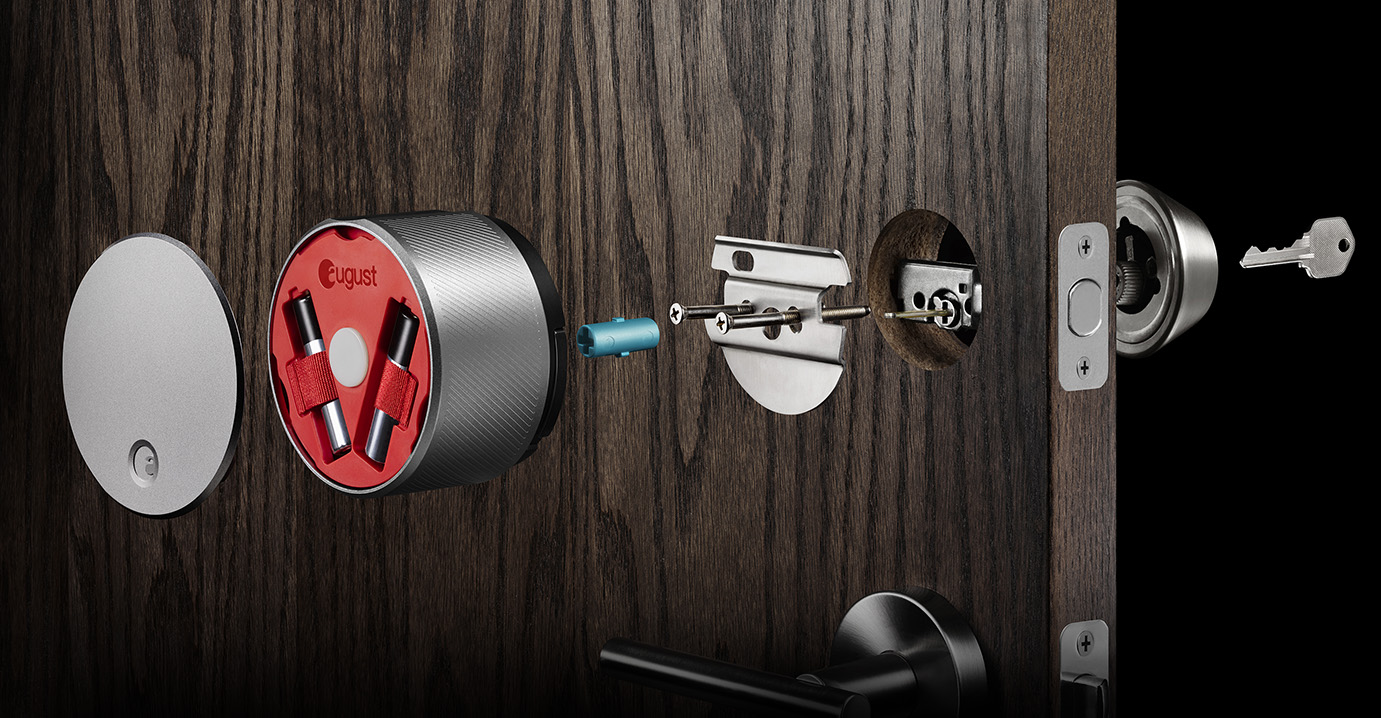
\includegraphics[width=0.9\textwidth]{graphics/august_2.jpg}
		\caption[Bestandteile eines August Smart Lock Pro]{Bestandteile eines August Smart Lock Pro\cite{August}}
		\label{fig:august1}
	\end{figure}
	
	\subsubsection{Typische Architekturen und Gemeinsamkeiten}
	\label{sec:sota_smart_locks_arch}
	    In den den doch sehr unterschiedlichen Produkten, die momentan auf dem freien Markt verfügbar sind oder bisher verfügbar waren, lassen sich trotz alledem einige Gemeinsamkeiten erkennen\cite{Ye2017,Fuller2017}. 
    	\noindent Generell besteht ein Smart Lock-System aus folgenden Bestandteilen (vgl. \fref{fig:sl_arch}):
    	\begin{enumerate}[noitemsep]
    		\item einem elektrischen Schloss oder einer elektronischen Erweiterung eines vorhandenen Schlosses
    		\item mindestens einem Nutzer, welcher durch sein Endgerät, meist ein Smartphone, identifiziert wird
    		\item einem oder mehreren herstellereigenen Servern
    		\item einem Webinterface
    		\item optional einem Zubehörgerät, welches dem Schloss als Gateway dient und es somit dem Schloss erlaubt mit dem Internet bzw. mit den Servern des Herstellers zu kommunizieren
    	\end{enumerate}
    
    	\begin{figure}[H]
			\centering
			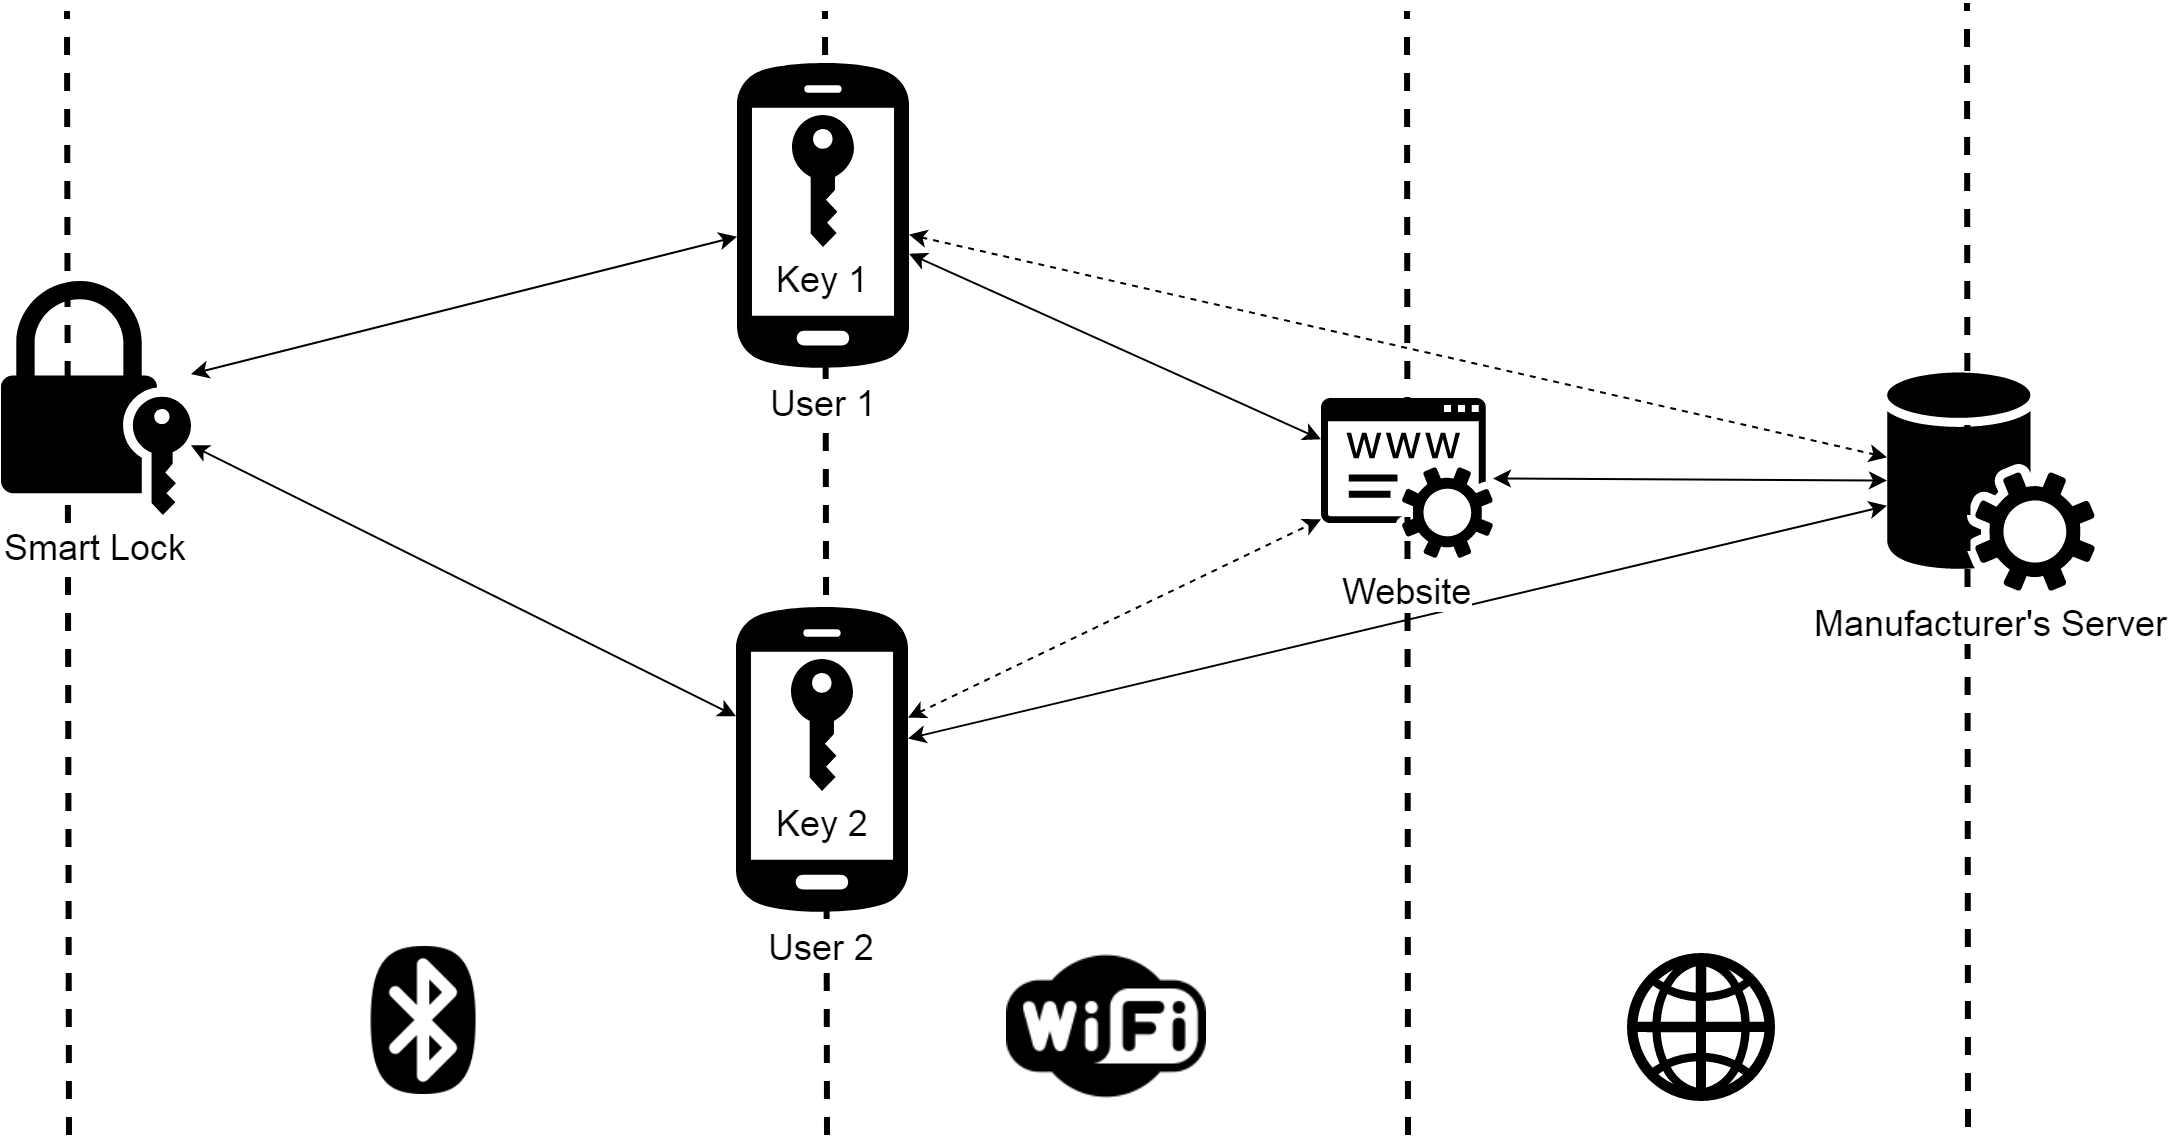
\includegraphics[width=\textwidth]{graphics/sl_arch.png}
			\caption[Beispiel eines Smart Lock-Systems]{Beispiel eines Smart Lock-Systems}
			\label{fig:sl_arch}
		\end{figure}
    	
	    \noindent Das Schloss selbst ist an der Außen- und/oder Innenseite einer Tür angebracht (vgl. \fref{fig:august1}) und erweitert ein vorhandenes Schloss elektronisch oder ist selbst in Form eines Vorhängeschlosses\cite{Ho2016}. 
		Zum System gehört in den meisten Fällen eine mobile Applikation für ein Smartphone zum Öffnen und Schließen des Schlosses, sowie zur Administration\cite{Fuller2017}. 
        Eher seltener beinhaltet das Produkt auch eine Weboberfläche, welche ebenfalls für administrative Aufgaben genutzt werden kann\cite{Ho2016}. 
		Es existiert ein herstellereigener (Remote-)Server, auf dem sich eine authoritative Liste aller Nutzer, sowie deren Rechte befindet. 
        Diese bildet die Grundlage zur Realisierung der Zugriffskontrolle.\cite{Fuller2017} 
        Das Öffnen und Schließen erfolgt primär elektronisch mittels eines Buttons per App.
        Alternativ lässt sich das Schloss entweder mit einem sogenannten ,,Keyfob`` 
        \footnote{ein Schlüsselanhänger, auf dem sich ein digitaler Schlüssel befindet} 
        oder einem physischen Schüssel öffnen\cite{Ho2016}. 
        Einige Modelle bieten auch eine Funktion, die die Tür automatisch öffnet sobald sich der Nutzer innerhalb eines selbst festgelegten Geofencing-Radius befindet. 
        (Bei Geofencing wird mittels \gls{gps} ein Ort festgelegt, um den ein virtueller Zaun gelegt wird. 
        Verlässt oder betritt der Nutzer den festgelegten Radius um den Ort, wird ein Trigger ausgelöst, dem beliebige Aktionen folgen können.) 
        \smallskip\\
        \noindent Sobald folgende Bedingungen gegeben sind, kann sich das Schloss automatisch öffnen: 
        \begin{itemize}[noitemsep]
        	\item automatisches Öffnen wurde vom Nutzer aktiviert
        	\item der Nutzer hat einen Ort für das Geofencing festgelegt
        	\item der Nutzer befindet sich in \gls{ble}-Reichweite, um über sein Smartphone mit dem Schloss kommunizieren zu können
        	\item der Nutzer ist berechtigt das Schloss zu öffnen
        \end{itemize}
    	Verlässt der Nutzer den Radius des Geofencings wieder, wird das Schloss automatisch verriegelt. 
    	\smallskip\\
		Ein optionales Zubehörgerät, welches in \fref{fig:sl_arch} nicht dargestellt wird, fungiert als Relay
		\footnote{leitet Nachrichten von mehreren Entitäten in einem Netzwerk (unverändert) weiter}
		, welches sich per \gls{ble} mit dem Schloss verbindet und über das W-LAN Heimnetzwerk des Nutzers mit dem Internet verbindet.
		
    \subsubsection{Typische Funktionen}
    \label{sec:sota_smart_locks_func}
		Um das Schloss zu kontrollieren installiert der Nutzer initial eine herstellerspezifische App auf seinem Smartphone und erstellt ein Nutzerkonto auf dem Server des Herstellers. 
		Danach pairt der Nutzer via \gls{ble} sein Gerät mit dem Schloss.\cite{Ho2016} 
		Die Identifikation der verschiedenen Nutzer für administrative Zwecke erfolgt entweder mittels E-Mailadresse oder Telefonnummer. 
		Aus technischer Sicht werden Nutzer anhand eines einzigartiger Schlüssel identifiziert, die der Besitzer des Schlosses nicht kennt.\cite{Fuller2017}\todo[color=orange]{nachlesen} 
		Die Smart Locks enthalten eine eingebaute Funktion, um Zugriffe zu protokollieren. 
		Dazu gehören Aktionen wie \cite{Fuller2017}:
		\begin{itemize}[noitemsep]
			\item von welchem Nutzer eine Funktion genutzt wurde, 
			\item der Zeitpunkt, an dem das Schloss elektronisch geöffnet oder geschlossen wurde,
			\item der Zeitpunkt, an dem das Schloss manuell geöffnet oder geschlossen wurde
			\item wann, wem und von wem Zugriff gewährt oder entzogen wurde
		\end{itemize}
	
	\subsubsection{Kommunikation}
	\label{sec:sota_smart_locks_comm}
	    \begin{figure}[H]
    		\centering
    		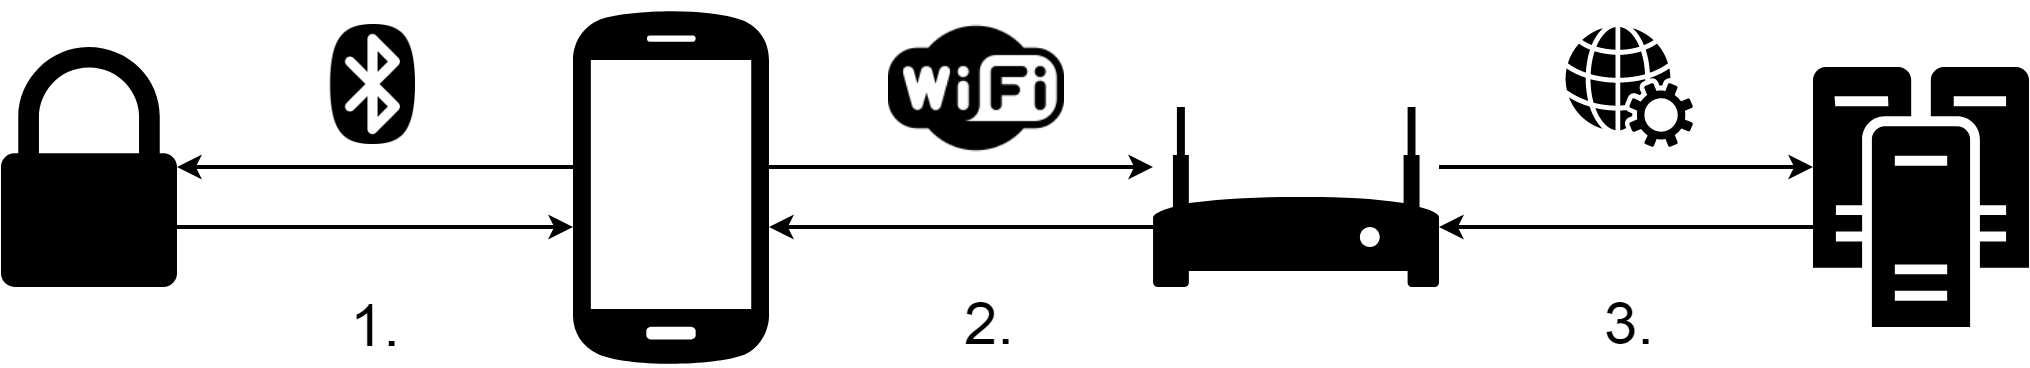
\includegraphics[width=0.9\textwidth]{graphics/gateway_arch.png}
    		\caption[Typische Architektur eines Smart Locks]{Typische Architektur, welche das Smartphone des Nutzers als Gateway/Proxy nutzt\cite{Ho2016}.}
    		\label{fig:gateway_arch}
    	\end{figure}
	    Nach \cite{Ho2016}:
        In \fref{fig:gateway_arch} erkennbar ist, dass das Smart Lock selbst hat keine direkte Verbindung zum Internet oder den Servern des Herstellers hat. 
        Das Endgerät des Nutzers übernimmt die Funktion eines Gateways für die Verbindung zum Internet und Proxys zur Übertragung von Informationen zwischen dem Smart Lock und den Servern des Herstellers. 
        Dies setzt voraus, dass sich das Endgerät in Kommunikationsreichweite von \gls{ble} befindet. 
        \smallskip\\
        Übertragen über \gls{ble} werden Informationen wie beispielsweise
        \begin{itemize}[noitemsep]
            \item Die in \fref{sec:sota_smart_locks_comm} beschriebenen Logdateien werden asynchron mit den Servern des Herstellers aktualisiert, sobald sich das Gerät des Nutzers in Reichweite des \gls{ble} befindet.
            \item Nachrichten mit Informationen über gewährten und entzogenen Nutzerrechten
            \item Athentifizierung des Smartphones des Nutzers 
        \end{itemize}
        
        \noindent Einige andere Modelle wie Lockitron\cite{lockitron} nutzen eine direkte Internetverbindung des Smart Locks zur Kommunikation mit den Servern des Herstellers. 
        Dabei baut das Schloss mittels eingebautem Wifi-Modem eine Verbindung mit dem Netzwerk des Nutzers auf und kommuniziert so mit den Servern. 
        Die übertragenen Informationen wie Rechtevergaben und Gerätezustand werden hier direkt über das Internet und nicht über lokale Kommunikation (wie \gls{ble}) übertragen. 

    \subsubsection{Sichereit}
    \label{sec:sota_smart_locks_sec}
        Häufig kommt für die Zugangskontrolle ein rollenbasiertes Konzept zum Einsatz. 
        Jeder Rolle werden bestimmte Rechte (vgl. \fref{tab:rbac}) zugeordnet.\cite{Ye2017,Ho2016,Fuller2017} 
		\begin{table}[H]
		    {\footnotesize
		    \centering
            \begin{tabular}{|m{0.114\textwidth}|m{0.114\textwidth}|m{0.114\textwidth}|m{0.114\textwidth}|m{0.114\textwidth}|m{0.114\textwidth}|m{0.114\textwidth}|}
            \hline
            \textbf{Rolle/Recht} & \textbf{Auto-Öffnen (de-)aktivieren} & \textbf{Lock/Unlock} & \textbf{Logdateien einsehen} & \textbf{Nutzer hinzufügen/löschen} & \textbf{Rollen\-verwal\-tung} & \textbf{Schloss kali\-brieren/zurück\-setzen} \\ \hline
            \textbf{Owner}      & \checkmark                   & \checkmark          & \checkmark           & \checkmark                         & \checkmark                    & \checkmark                           \\ \hline
            \textbf{Resident}   & \checkmark                   & \checkmark          & ~                    & ~                                  & ~                             & ~                                    \\ \hline
            \textbf{Guest}      & \checkmark                   & \checkmark          & ~                    & ~                                  & ~                             & ~                                    \\ \hline
            \end{tabular}
            }
            \caption[Rollenbasierte Zugangskontrolle bei Smart Locks]{Beispiel einer rollenbasierten Zugriffskontrolle bei Smart Locks}
            \label{tab:rbac}
        \end{table}
		\normalsize
		\noindent In \fref{tab:rbac} nicht angegeben, aber dennoch für alle Rollen gültig: Jeder kann seinen eigenen Account löschen. 
		\begin{description}
		    \item [Owner] Die Rolle des Owners wird jenem Gerät vergeben, das sich nach Installation bzw. nach Zurücksetzen des Smart Locks als erstes mittels \gls{ble} verbindet. 
   		        Auf diesem Wege wird die Owner-Rolle nur einmal vergeben. 
   		        Bei Wechsel des Besitzers muss das Smart Lock zurückgesetzt werden. 
   		        Ein Owner kann allerdings auch die Rolle des Owner an andere Nutzer weitergeben, sowie diese wieder entziehen. 
   		        Um die Rechte eines Owners bei einem verlorenen oder gestohlenen zu entziehen, wird entweder eine ,,Lost Phone``-Funktion angeboten oder ein anderer Nutzer mit der Rolle des Owners entzieht dem nicht mehr vorhandenen Gerät die Rolle. 
   		        Der Owner kann das Schloss auch ohne Internetverbindung öffnen/schließen. 
   	        \item [Resident] Ein Bewohner kann das Schloss öffnen oder schließen. 
   	            Sollte die automatische Öffnen/Schließen-Funktion aktiviert werden, wird auch bei einem Bewohner das Schloss automatisch geöffnet und geschlossen. 
   	            Bewohner und Gäste müssen sich vor der Kommunikation mit dem Schloss gegenüber der dem Server des Herstellers autorisieren lassen.
   	        \item [Guest] Der Gast unterscheidet sich von einem Bewohner lediglich darin, dass er nur innerhalb eines begrenzten Zeitraums Zugang hat. 
                Der Zeitraum des Zugangs wird durch einen Owner festgelegt.
		\end{description}
        
		\paragraph{Secret Keys}\hspace{0pt}\smallskip\\
		Jede Bluetooth-Verbindungssession bekommmt einen eigenen einzigartigen \gls{sk}, welcher für Owner und Guest/Resident unterschiedlich entsteht.
		Dieser wird verwendet, um Nachrichten zwischen dem Schloss und dem Smartphone des Nutzers mit dem Verschlüsselungsalgorithmus \gls{aes} zu ver- und entschlüsseln. 
		Voraussetzung für das Protokoll, welches den Session Key erstellt ist, dass bereits im Voraus das Schloss und entweder die Webserver des Herstellers oder das Smartphone des Nutzers einen Secret Key teilen. 
		Dieser Secret Key ist beipsielsweise das Passwort, das der Nutzer während seiner Anmeldung in der App verwendet. 
		In dem Smart Lock von August können insgesamt 256 Schlüssel (von 0 bis 255 nummeriert, je einen pro Nutzer des Schlosses) gespeichert werden, wobei Nummer 0 besondere Privilegien hat und als ,,Firmware Key`` angesehen wird.\cite{Jmaxxz2016,Fuller2017} 
		Der Key 0 wird dazu genutzt die anderen Keys zu übertragen und ist hardcoded. 
        Die restlichen 255 Keys sind ,,offline Keys``, die zur Initialisierung einer Bluetooth-Session verwendet werden, sollte der Nutzer nicht mit dem Internet verbunden sein.\cite{Fuller2017}
        
		\begin{figure}[!htbp]
    		\centering
    		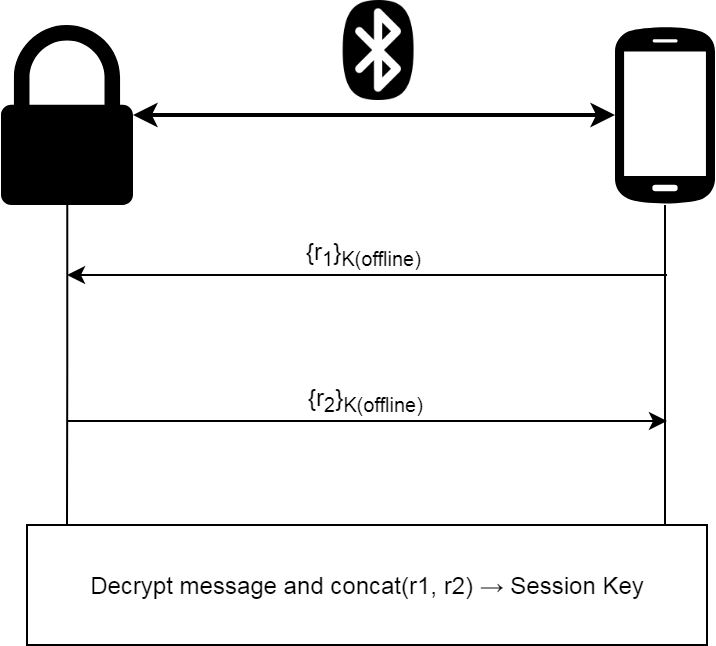
\includegraphics[width=0.6\textwidth]{graphics/owner_key.png}
    		\caption[Generierung eines Session Keys mittels Offline Key]{Ablauf der Generierung eines \gls{sk} mittels offline Key\cite{Fuller2017}}
    		\label{fig:owner_key}
    	\end{figure}
		
		\noindent\fref{fig:owner_key}\todo[color=yellow]{bessere Überleitung}:
        \begin{enumerate}[noitemsep]
            \item das Smartphone sendet zufällige 64 Bit an das Schloss, welche mit dem offline Keys des Smartphones verschlüsselt werden, an das Schloss
            \item das Schloss sendet 64 zufällige Bits, die mit dem offline Key des Smartphones verschlüsselt sind, an das Smartphone zurück
            \item das Schloss und das Smartphone entschlüsseln die jeweils erhaltene Nachricht und konkatinieren beide Nachrichten zu einer neuen 128-Bit langen Folge, die im weiteren Verlauf als \gls{aes}-Key zur Verschlüsselung der Session genutzt wird
        \end{enumerate}
        
        \noindent Gäste, welche keinen ,,offline Key`` zugewiesen bekommen, kommunizieren mit dem Webserver (vgl. \fref{fig:online_key}):\todo[color=orange]{nachlesen}
        
        \begin{figure}[!htbp]
    		\centering
    		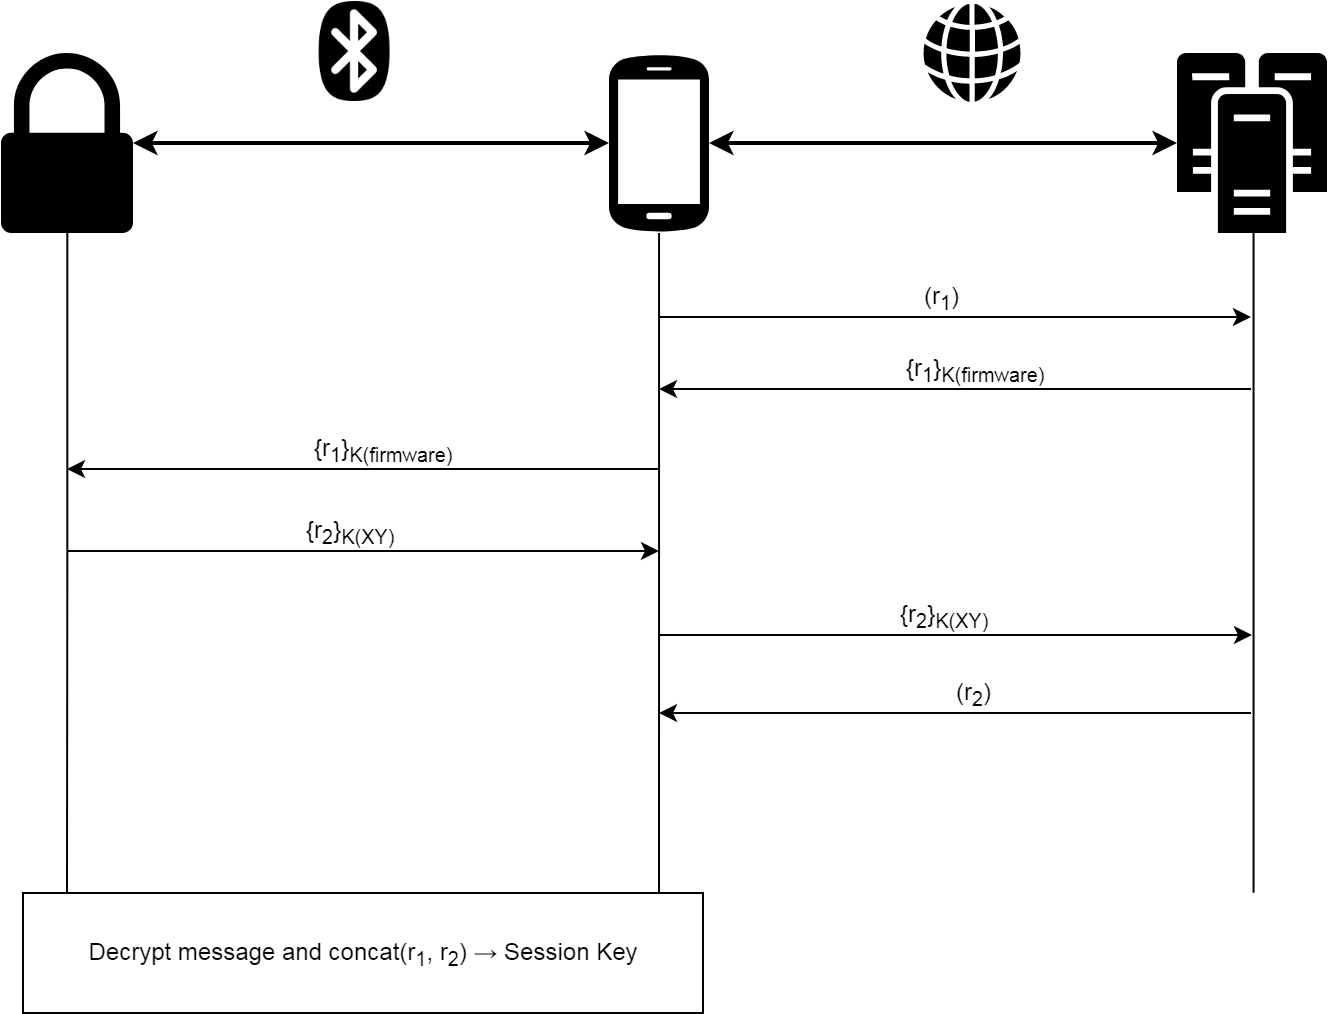
\includegraphics[width=0.9\textwidth]{graphics/online_key.png}
    		\caption[Generierung eines Session Keys ohne Offline Key]{Ablauf der Generierung eines \gls{sk} ohne offline Key\cite{Fuller2017}}
    		\label{fig:online_key}
    	\end{figure}
        
        \begin{enumerate}[noitemsep]
            \item das Smartphone des Gasts sendet 64 zufällige Bits als Klartext an den Server
            \item der Server verschlüsselt diese 64 Bits mit dem Firmware Key und sendet die verschlüsselten Bits als Nachricht an den Gast zurück
            \item der Gast leitet den Ciphertext, welcher von dem Server empfangen wurde, an das Schloss weiter
            \item das Schloss sendet 64 Bits mit XY\todo[color=orange]{nachlesen} verschlüsselt an den Gast, welcher diesen Ciphertext an den Server weiterleitet
            \item Der Server entschlüsselt die Nachricht und sendet sie als Klartext per SSL an den Gast
            \item das Schloss und der Gast konkatenieren beide 64-Bit langen Folgen zu einem 128-Bit Schlüssel, welcher als Session Key verwendet wird
        \end{enumerate}
